\section{Results}
\paragraph{}
In this section, we present the evaluation results for the word and character recognition models. The purpose is to assess the performance of each model and gain insights into their effectiveness.
\subsection{Word Recognition Results}
\paragraph{}
The word recognition model was evaluated using a comprehensive set of word samples. The model achieved an accuracy of 94.63\% on the test dataset. The confusion matrix, depicted in Figure \ref{fig:words_confusion_matrix}, shows the distribution of predicted labels versus the true labels for each word class.
\paragraph{}
From the confusion matrix, we can observe that the model performs remarkably well, with most of the samples being correctly classified. There are only slight errors in some cases. However, overall, the model demonstrates high accuracy and precision.
\paragraph{}
To gain a comprehensive understanding of the word recognition model's performance, we present the classification report in Figure \ref{fig:words_classification_report}.
\paragraph{}
The classification report provides insights into the precision, recall, and F1 score for each word class. The macro average precision, recall, and F1 score for the word recognition model are 94\%, 95\%, and 95\%, respectively. These results indicate the model's strong performance in correctly recognizing the majority of the word classes.
 \ref{tab:words_classification_report}.
\subsection{Character Recognition Results}
\paragraph{}
Moving on to character recognition, the model achieved an accuracy of 95.03\% on the test dataset. The confusion matrix, shown in Figure \ref{fig:characters_confusion_matrix}, illustrates the predicted labels versus the true labels for each character class.
\paragraph{}
Similar to the word recognition model, the confusion matrix for the character recognition model demonstrates excellent performance, with minimal errors. The model accurately recognizes the majority of the characters, with only slight confusion between similar characters like "u" and "v".
\paragraph{}
To gain a comprehensive understanding of the character recognition model's performance, we present the classification report in Figure \ref{tab:characters_classification_report}.
\paragraph{}
The classification report presents the precision, recall, and F1 score for each character class. The average precision, recall, and F1 score for the character recognition model are 95\% for all of them. These results indicate the model's high accuracy in correctly identifying the majority of the character classes.
\paragraph{}
In summary, both the word and character recognition models demonstrate excellent performance with an accuracy of 94.63\% and 95.03\% respectively. The confusion matrices reveal minimal errors, while the classification reports confirm the models' precision, recall, and F1 score across various word and character classes. These results indicate the effectiveness and reliability of the implemented models in \ac{slr}.
\begin{figure}[h]
	\centering
	\begin{subfigure}[b]{0.6\textwidth}
		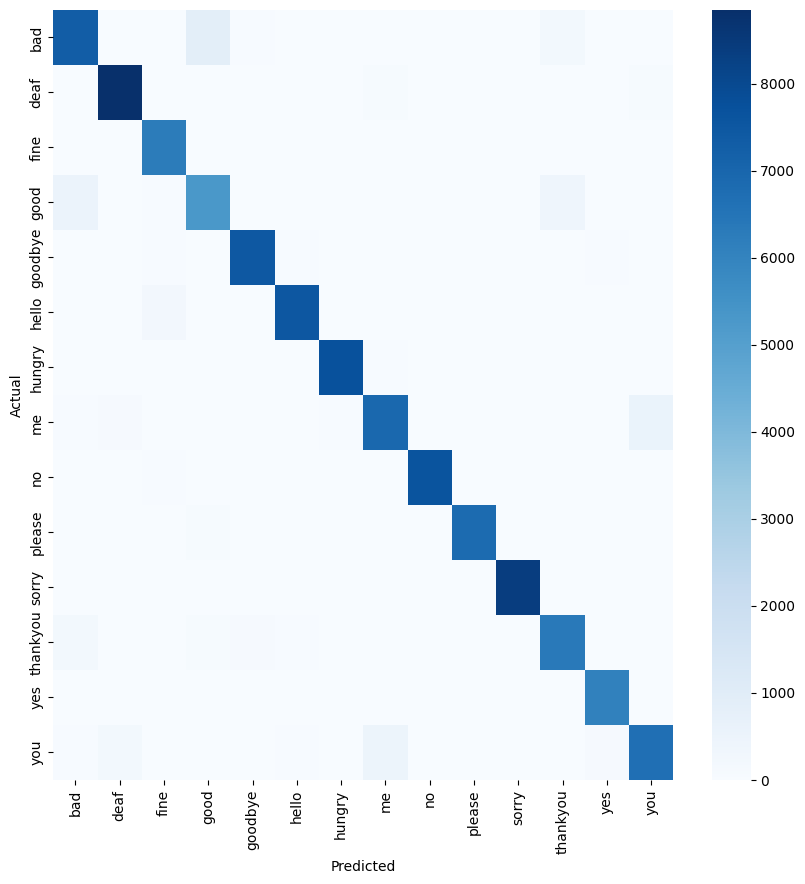
\includegraphics[width=\textwidth]{images/confusion_matrix_words}
		\caption{Confusion matrix for the word recognition model.}
		\label{fig:words_confusion_matrix}
	\end{subfigure}
	\begin{subfigure}[b]{0.6\textwidth}
		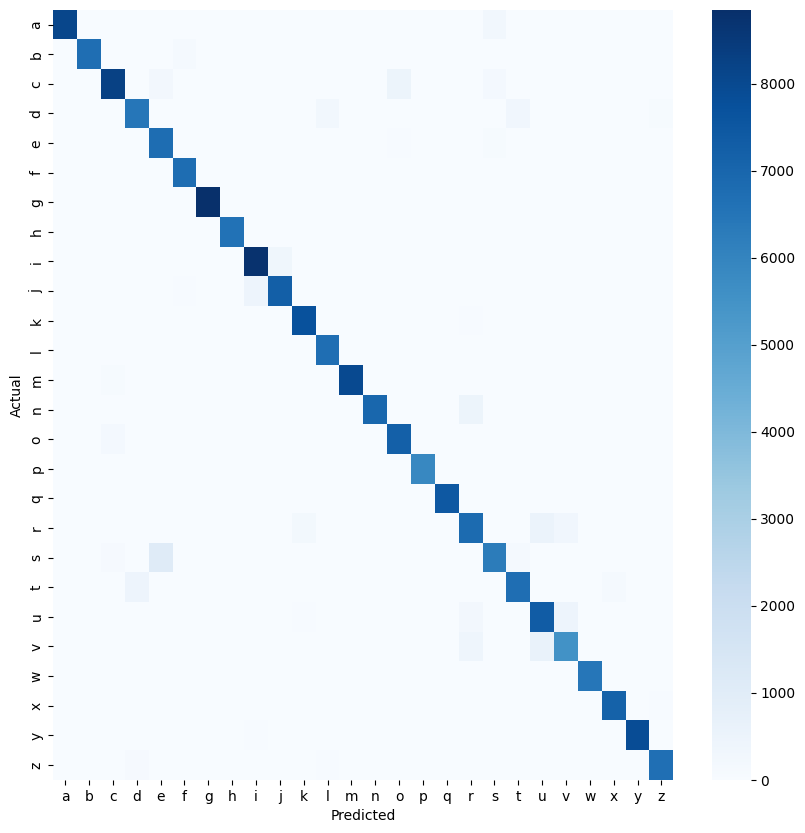
\includegraphics[width=\textwidth]{images/confusion_matrix_characters}
		\caption{Confusion matrix for character recognition model}
		\label{fig:characters_confusion_matrix}
	\end{subfigure}
	\caption{Confusion matrices}
	\label{fig:confusion_matrices}
\end{figure}
\begin{table}[h]
	\centering
	\begin{tabular}{|c|c|c|c|c|}
		\hline
		& precision & recall & f1-score & support \\
		\hline
		bad & 0.89 & 0.86 & 0.87 & 8550 \\
		\hline
		deaf & 0.96 & 0.98 & 0.97 & 9000 \\
		\hline
		fine & 0.93 & 0.99 & 0.96 & 6300 \\
		\hline
		good & 0.82 & 0.84 & 0.83 & 6300 \\
		\hline
		goodbye & 0.98 & 0.98 & 0.98 & 7650 \\
		\hline
		hello & 0.98 & 0.96 & 0.97 & 7800 \\
		\hline
		hungry & 0.99 & 0.99 & 0.99 & 7800 \\
		\hline
		me & 0.91 & 0.89 & 0.90 & 7800 \\
		\hline
		no & 1.00 & 0.99 & 1.00 & 7650 \\
		\hline
		please & 0.99 & 0.97 & 0.98 & 7050 \\
		\hline
		sorry & 0.99 & 1.00 & 1.00 & 8400 \\
		\hline
		thankyou & 0.90 & 0.93 & 0.91 & 6900 \\
		\hline
		yes & 0.97 & 0.99 & 0.98 & 6150 \\
		\hline
		you & 0.91 & 0.87 & 0.89 & 7650 \\
		\hline
		accuracy & - & - & 0.95 & 105000 \\
		\hline
		macro avg & 0.94 & 0.95 & 0.95 & 105000 \\
		\hline
	\end{tabular}
	\caption{Words classification report}
	\label{tab:words_classification_report}
\end{table}
\begin{table}[h]
	\centering
	\begin{tabular}{|c|c|c|c|c|}
		\hline
		& precision & recall & f1-score & support \\
		\hline
		a & 1.00 & 0.96 & 0.98 & 8400 \\
		\hline
		b& 1.00 & 0.98 & 0.99 & 6900 \\
		\hline
		c & 0.95 & 0.89 & 0.92 & 9300 \\
		\hline
		d & 0.91 & 0.89 & 0.90 & 7200 \\
		\hline
		e & 0.83 & 0.98 & 0.90 & 6900 \\
		\hline
		f & 0.97 & 1.00 & 0.99 & 6750 \\
		\hline
		g & 1.00 & 1.00 & 1.00 & 8850 \\
		\hline
		h & 1.000 & 1.00 & 1.00 & 6600 \\
		\hline
		i & 0.94 & 0.96 & 0.95 & 9150 \\
		\hline
		j & 0.95 & 0.93 & 0.94 & 7800 \\
		\hline
		k & 0.96 & 0.99 & 0.97 & 7800 \\
		\hline
		l & 0.95 & 1.00 & 0.97 & 6750 \\
		\hline
		m & 1.00 & 0.99 & 0.99 & 8100 \\
		\hline
		n & 0.99 & 0.93 & 0.96 & 7500 \\
		\hline
		o & 0.93 & 0.96 & 0.94 & 7500 \\
		\hline
		p & 1.00 & 1.00 & 1.00 & 5850 \\
		\hline
		q & 1.00 & 1.00 & 1.00 & 7500 \\
		\hline
		r & 0.85 & 0.86 & 0.85 & 7950 \\
		\hline
		s & 0.91 & 0.82 & 0.86 & 7650 \\
		\hline
		t & 0.93 & 0.91 & 0.92 & 7350 \\
		\hline
		u & 0.86 & 0.91 & 0.88 & 8100 \\
		\hline
		v & 0.87 & 0.83 & 0.85 & 6600 \\
		\hline
		w & 1.00 & 1.00 & 1.00 & 6450 \\
		\hline
		x & 0.97 & 0.99 & 0.98 & 7200 \\
		\hline
		y & 0.99 & 0.99 & 0.99 & 7950 \\
		\hline
		z & 0.98 & 0.97 & 0.97 & 6900 \\
		\hline
		accuracy & - & - & 0.95 & 195000 \\
		\hline
		macro avg & 0.95 & 0.95 & 0.95 & 195000 \\
		\hline
	\end{tabular}
	\caption{Characters classification report}
	\label{tab:characters_classification_report}
\end{table}